\documentclass[11pt]{beamer}
\setbeamertemplate{navigation symbols}{}%remove navigation symbols
\usepackage{booktabs}
\usepackage{hyperref}
%\usepackage{curvedarrows}  
\usepackage{cutwin}  
\usepackage{lipsum}  
\usepackage{subcaption}
\captionsetup{compatibility=false}
\def\leq{\leqslant}  
\def\geq{\geqslant} 
%\usepackage{subfig}
\usepackage{tcolorbox}

\usefonttheme{professionalfonts}
%\usefonttheme{serif}

%\usepackage{fontspec}
%\usepackage{kantlipsum}
\setbeamerfont{note page}{family*=pplx,size=\footnotesize}
\useoutertheme{infolines}

\usepackage[framemethod=tikz]{mdframed}
\usetikzlibrary{shadows}
\usepackage{pdfpages}
\newmdenv[shadow=true,shadowcolor=black,font=\sffamily,rightmargin=8pt]{shadedbox}
\usepackage{pifont,xcolor}% http://ctan.org/pkg/{pifont,xcolor}
\definecolor{myblue}{RGB}{49,54,149}
\definecolor{myred}{RGB}{165,0,38}
\usepackage{graphicx}
\usepackage{caption}
\newcommand{\lenitem}[2][.55\linewidth]{\parbox[t]{#1}{#2\strut \strut}}

\usetheme{Frankfurt}

   \usefonttheme{professionalfonts} 
\newenvironment{variableblock}[3]{%
  \setbeamercolor{block body}{#2}
  \setbeamercolor{block title}{#3}
  \begin{block}{#1}}{\end{block}}
\usecolortheme{dove}
\usepackage{fancybox}
\setbeamercolor{block title}{bg=white,fg=black}
\newenvironment{fminipage}%
{\begin{Sbox}\begin{minipage}}%
{\end{minipage}\end{Sbox}\fbox{\TheSbox}}

\newcommand{\itemcolor}[1]{% Update list item colour
  \renewcommand{\makelabel}[1]{\color{#1}\hfil ##1}}

\newcounter{tmpc}
%\usefonttheme{structuresmallcapsserif}
\setbeamercolor{section in head/foot}{fg=black, bg=white}
\setbeamercolor{enumerate item}{ fg=red}
\setbeamertemplate{frametitle}
{
    \nointerlineskip
    \begin{beamercolorbox}[sep=0.3cm,ht=1.8em,wd=\paperwidth]{frametitle}
        \vbox{}\vskip-3ex%
        \strut\insertframetitle\strut
        \vskip-1.2ex%
    \end{beamercolorbox}
}
\addtobeamertemplate{frametitle}{\vskip0.5ex}{}
\makeatletter
\setbeamertemplate{footline}
{
  \leavevmode%
  \hbox{%
  \begin{beamercolorbox}[wd=.875 \paperwidth,ht=2.25ex,dp=1ex,left]{section in head/foot}%
    \usebeamerfont{author in head/foot}\quad \quad \insertshorttitle
 \end{beamercolorbox}%
 \begin{beamercolorbox}[wd=.125\paperwidth,ht=2.25ex,dp=1ex,right]{section in head/foot}%
    \usebeamerfont{date in head/foot} \quad \quad
    \insertframenumber{} / \inserttotalframenumber\hspace*{2ex} 
  \end{beamercolorbox}}%
  \vskip0pt%
}
\let\@@magyar@captionfix\relax
\makeatother

\def\mf{
\begin{itemize}
\item Item
\end{itemize}
}
%\setbeamercolor{itemize item}{fg=yellow,bg=white}
%\setbeamertemplate{itemize items}[circle]
\setbeamercolor{enumerate item}{ fg=red}
\setbeamercolor{item projected}{bg=myblue}

\begin{document}

\section{Title Page}
\subsection{}
\small
\title{Public Procurement from the Private Sector\vspace{-.2in}} 
\author{Charles Rahal\\ Department of Sociology and Nuffield College \\ University of Oxford \\ \vspace{0.1in} 
\color{myblue}ADRN Conference\\\color{black}Queens University, 22nd June, 2018}
 \date{}
\frame{\titlepage 
\begin{center}
 \vspace{-0.7in}
\begin{figure}
\centering
\begin{minipage}{.5\textwidth}
  \centering
  
\includegraphics[width=.35\linewidth]{oxfordlogo.png}
  \label{fig:test1}
\end{minipage}\hspace{-.35in}
\begin{minipage}{.5\textwidth}
  \centering
  
\includegraphics[width=.7\linewidth]{BAlogo.jpg}
  \label{fig:test2}
\end{minipage}
\end{figure}\vspace{0.05in}
\begin{center}
\footnotesize
Contains public sector information licensed under the Open Government Licence v3.0.\\ \vspace{0.05in}
Open Source (MIT): \color{myred}\url{https://github.com/crahal/centgovspend}\color{black}\\ \vspace{0.05in}
Please note this is \color{myblue}\texttt{extremely} \color{black}preliminary work!
\end{center}


 \end{center}
}
\section{Introduction}
\frame{
\frametitle{Introducting a Lesser Known Administrative Data Type}
\begin{itemize}
\footnotesize
\item Today we'll talk about transparency and public payments data (`Open Data').\vspace{0.05in}
\item Coalition (31/05/2010) enforced accountability and aimed to reduce costs.\vspace{0.05in}
\item Each department now has a Minister responsible for transparency issues.\vspace{0.05in}
\item Range of measures: $\pounds$10k contracts, gifts, gender pay gaps, hospitality, etc.\vspace{0.05in}
\item We're going to focus on central government spending over $\pounds$25k.\vspace{0.05in}
\begin{itemize}
\item In particular: transaction level data across ministerial and non-ministerial bodies.\vspace{0.05in}
\end{itemize}
\item This policy relates to all central govermnent including, NHS, NDPBs, etc.\vspace{0.05in}
\item Datasource largely untapped: \textbf{huge} in magnitude -- UK spends $\pounds$800bn p.a.\vspace{0.05in}
\item It would be great to know where that money goes, right?\vspace{0.05in}
\end{itemize}
}


\begin{frame}
\frametitle{Mostly NGO and With Limited Academic Contributions}
       \begin{columns}
          \column{0.425\linewidth}
             \centering
             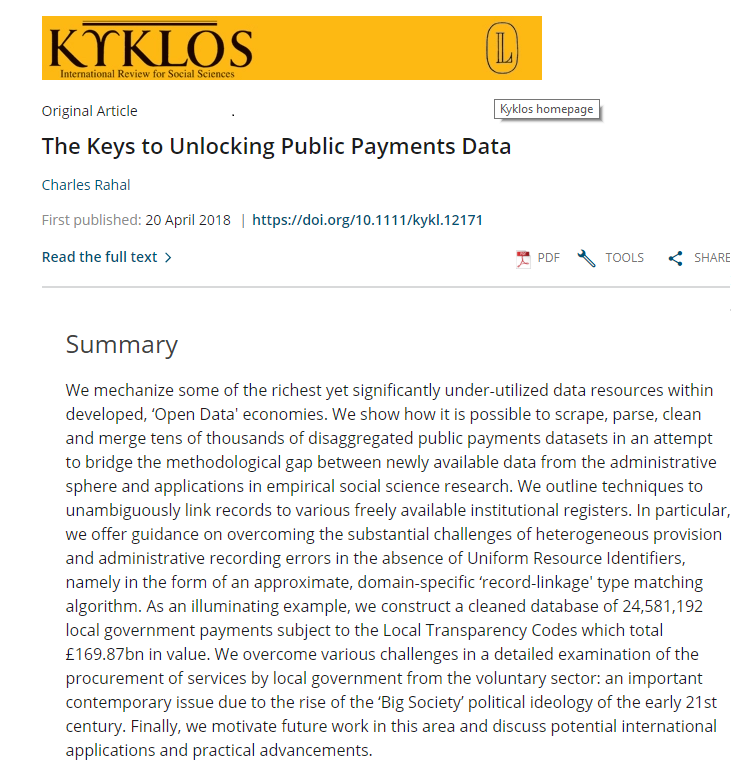
\includegraphics[height=6cm, width = 5.5cm]{kyklos.png}
           \column{0.575\linewidth}
\begin{itemize}
\footnotesize
\item Academic work limited to this one paper (?)\vspace{0.025in}
\item Todays content builds on an earlier prototype which creates payments databases from LA's subject to the LATC.\vspace{0.025in}
\item Most civic tech projects ran out of steam.\vspace{0.025in}
\item OCP are an integral player internationally.\vspace{0.025in}
\item Some collaboration with TI.\vspace{0.025in}
\item Spend Network: excellent open data business with a pricing structure.\vspace{0.025in}
\item This project aims to make software (\texttt{centgovspend}) to produce a bulk download for academic analysis possible.\vspace{0.025in}
\end{itemize}
         \end{columns} 
    \end{frame}


\section{Data}
\frame{
\frametitle{Data}
\begin{itemize}
\item Data origination is convoluted for multiple reasons:\vspace{0.05in}
\begin{enumerate}
\setbeamercolor{enumerate subitem}{fg=red!80!black}
\setbeamertemplate{enumerate items}[default]
\footnotesize
\item Fragmented: hosted on gov.uk, data.gov.uk \textit{or} their department sites.\vspace{0.05in}
\item Untimely: sporadically updated (at best) -- \textit{should be} within one month\vspace{0.05in}
\item Heterogeous: despite guidelines, providers supply in different formats.\vspace{0.05in}
\item Messy: requires substantial cleaning.\vspace{0.025in}
\item User-input: requires verification (boo) or automated reconciliation (yay).\vspace{0.075in}
\end{enumerate}
\item In theory: 45 (non-)ministerial departments, 8 years, monthly = 4,320 files.\\ \vspace{0.1in}
\item Most commonly available in \texttt{.csv}, {.xls}, \texttt{.xlsx} (`3$^*$' and `2$^*$' files): none of the .pdfs (`1$^*$') which plague NHS and LA data! This leads to a clean tool.\vspace{0.1in}
\item Spending data involved made available under an Open Government License.
\end{itemize}
}

\section{centgovspend}
\frame{
\frametitle{Introducing centgovspend}
\begin{itemize}
\item \color{myred}\texttt{centgovspend}\color{black}: a modular open source library available on GitHub.\vspace{0.025in}
\item Updated quarterly (next: 01/07/2018) for new sources and edge cases.\vspace{0.05in}
\item Different modules and functions...:\vspace{0.05in}
\begin{enumerate}
\setbeamercolor{enumerate subitem}{fg=red!80!black}
\setbeamertemplate{enumerate items}[default]
\item Scrape all ministerial and non-ministerial locations for data.\vspace{0.05in}
\item Clean files generally (e.g. dupes, blank rows) and harmonizes headers.\vspace{0.05in}
\item Parse into a database of cleaned payments, retaining seven key fields.\vspace{0.05in}
\item Remove problematic suppliers (e.g. `redacted', `various' and variants).\vspace{0.05in}
\item Evaluates the scraping procedure.\vspace{0.05in}
\item Moves onto reconciliation...\vspace{0.1in}
\end{enumerate}
\end{itemize}
}

\begin{frame}[fragile]
\frametitle{Evaluating the Scrape and Parse}
\begin{verbatim}
** Evaluating the merged Dataset!**
** We have 3291682 total rows of data to begin.
We lose 11412 rows due to nulls in supplier\amount\bad dates.
Dropped 36361 redacted payments
Dropped redacted payments worth £201.08bn
We identified 247 redacted Suppliers
Dropped 14 "various" payments
Dropped "various" payments worth £50.05bn
We identified 1 "various" Suppliers
Dropping 309653 potential duplicates
** This spending totals £998.68bn.
** This is from a total of 2,719,026 payments. 
** We merge from across 38 departments.
** This data comes from: 2179 files.
** We have: 60,597 unique supplier strings.
Cleaned file at: output\All_Merged_Unmatched.csv
\end{verbatim}
\end{frame}



\frame{
\frametitle{Results vis a vis Policy timeline}
\begin{figure}
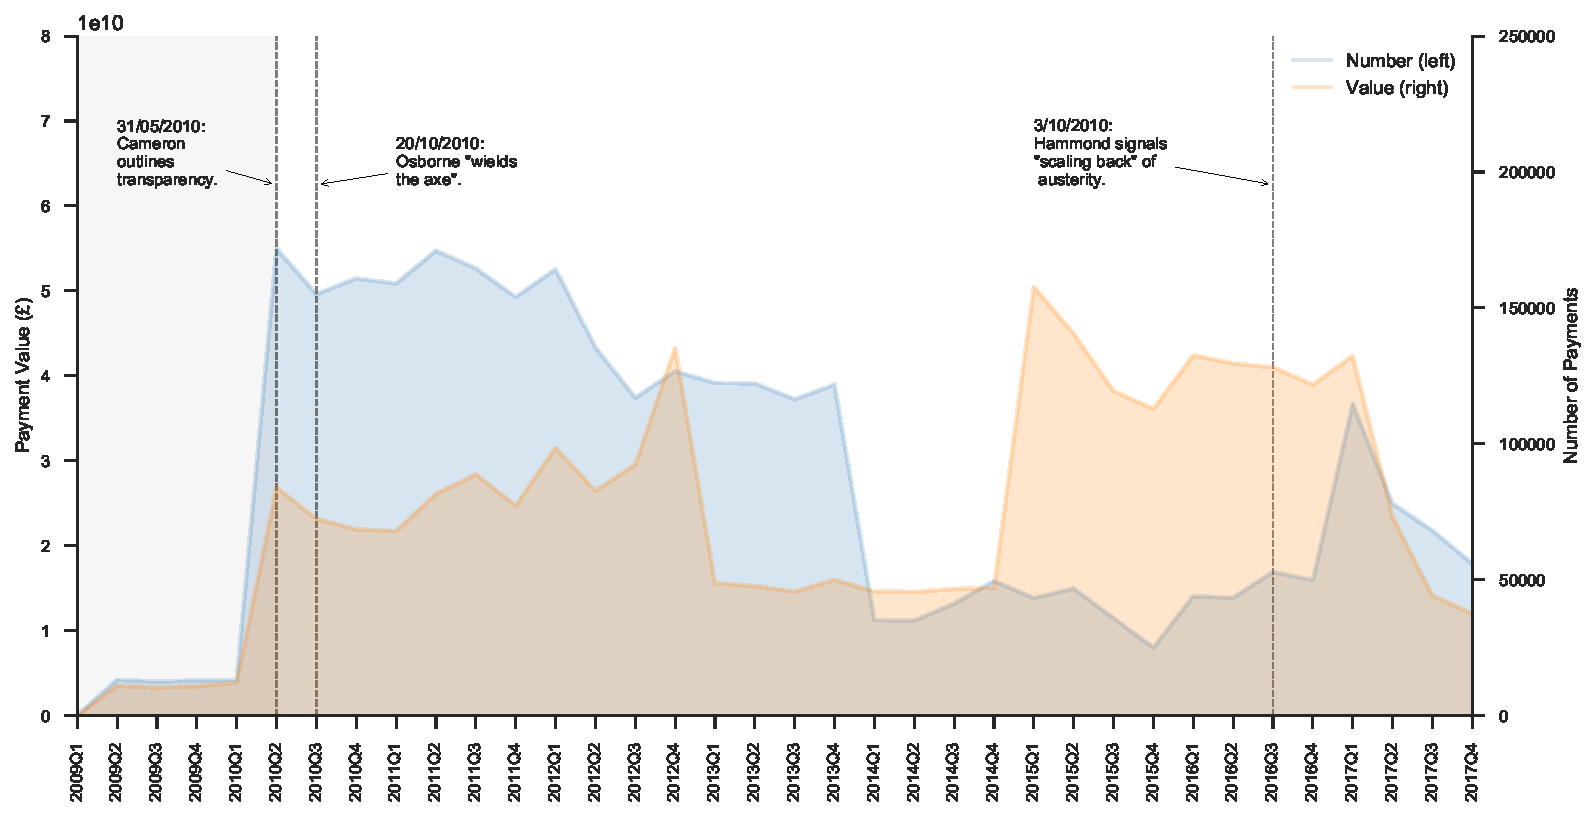
\includegraphics[width=\textwidth, angle=0]{timeline.pdf}
\end{figure}
}

\frame{
\frametitle{Methods: Reconciliation}
\begin{itemize}
\item Before analysis, we need an algorithm for reconciling supplier names.\vspace{0.1in}
\item With a simple exact match strategy for groupings, how to know `23RED' and `23RED LTD'  both relate to a `23RED LIMITED'?\vspace{0.01in}
\item We design modules to reconcile via the OpenCorporates API\vspace{0.025in}
\begin{itemize}
\item We write code to bypass OpenRefine and hit the OC REST API directly\vspace{0.025in}
\item OC API is based on a normalized supplier name with Elastic Search\vspace{0.025in}
\end{itemize}
\item For each unique company reconciled, request from Companies House API:\vspace{0.05in}
\begin{enumerate}
\setbeamercolor{enumerate subitem}{fg=red!80!black}
\setbeamertemplate{enumerate items}[default]
\item Basic company details.\vspace{0.05in}
\item Information on all company officers.\vspace{0.05in}
\item Information on persons of signifciant control (PSC).\vspace{0.05in}
\end{enumerate}
\end{itemize}
}


\begin{frame}[fragile]
\frametitle{Manual Verification and Automated Safematch Algorithms}
\begin{figure}
\centering
\begin{subfigure}{.5\textwidth}
  \centering
    \caption{Manual Verification}
  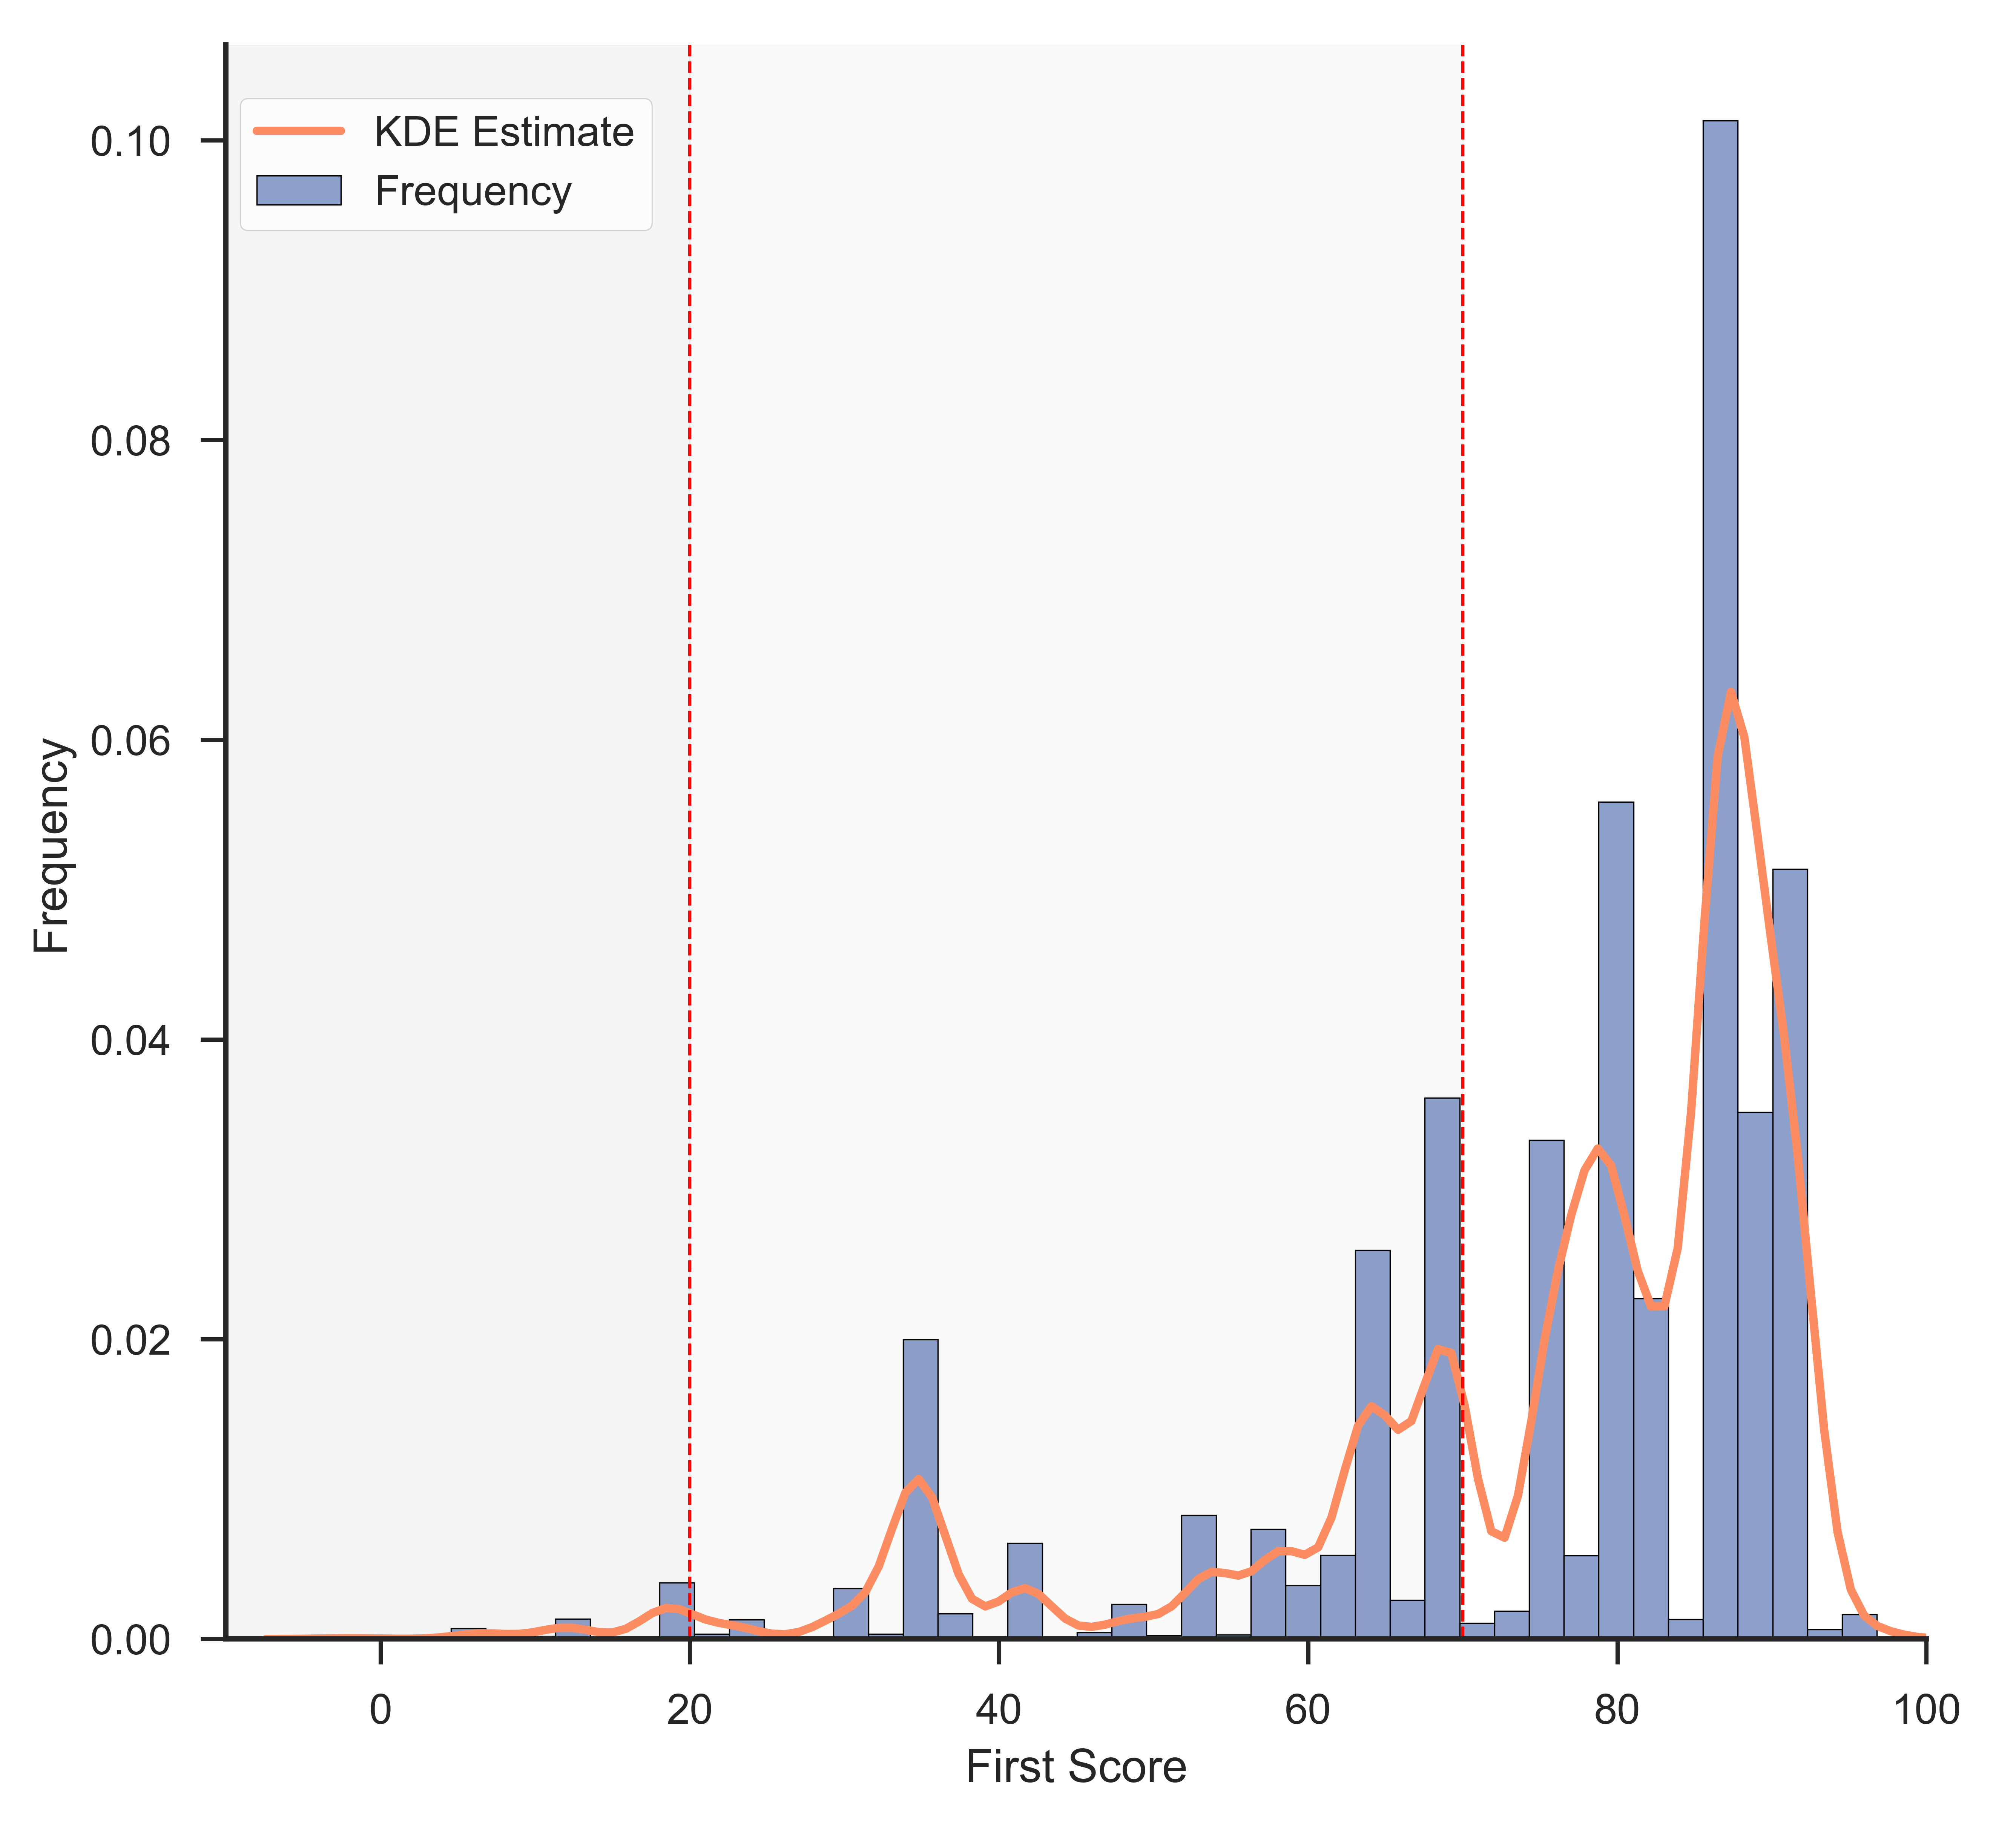
\includegraphics[width=.8\linewidth]{image1-0.png}
  \label{fig:sub1}
\end{subfigure}%
\begin{subfigure}{.5\textwidth}
  \centering
    \caption{Automated Safematch}
  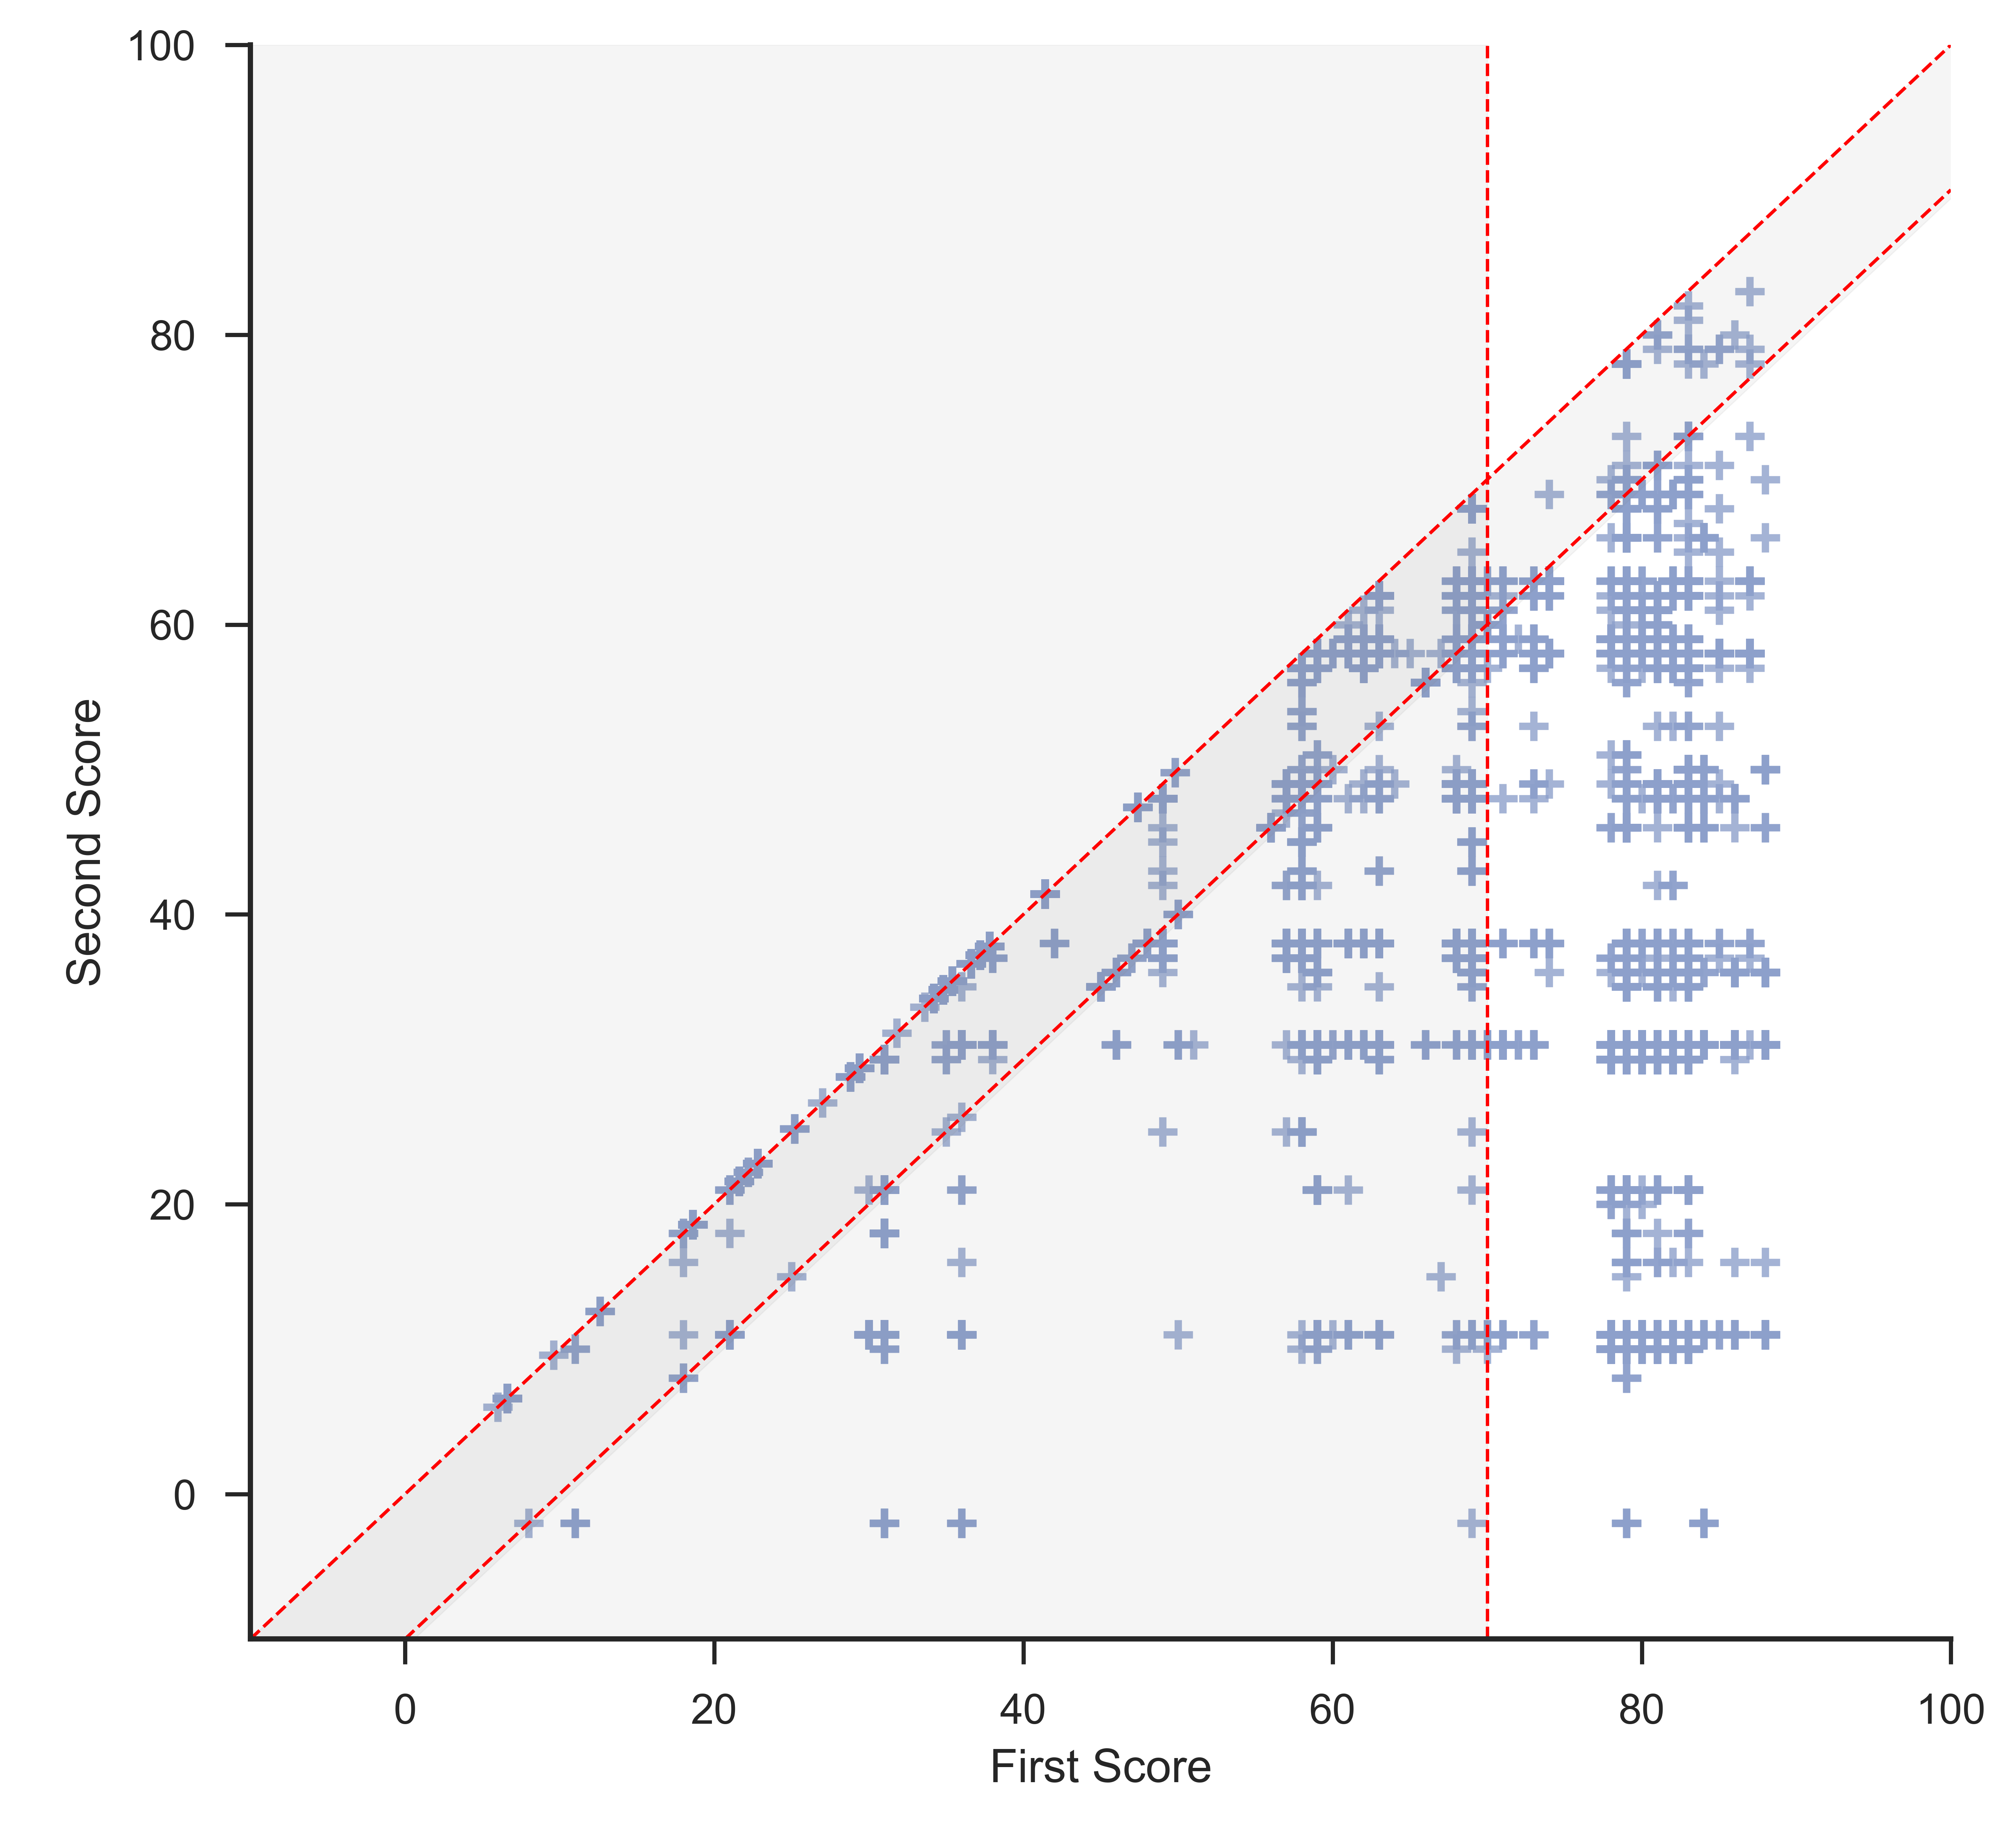
\includegraphics[width=.8\linewidth]{image1-1.png}
  \label{fig:sub2}
\end{subfigure}
\label{fig:test}
\end{figure}\scriptsize
We provide two functions for verifying the OC matches. From \texttt{automated safematch}:
\begin{verbatim}
    We matched 1443852 out of 2719026 payments in total (53.1%).
    We matched £118869981782 out of £998678528765 value in total 11%).
    We matched 18963 out of 60597 unique suppliers in total (31.29%).
\end{verbatim}
\end{frame}


\section{Cleaned Database}
\frame{
\frametitle{Aggregating Spend Across Standard Industry Classifiers}
\begin{figure}
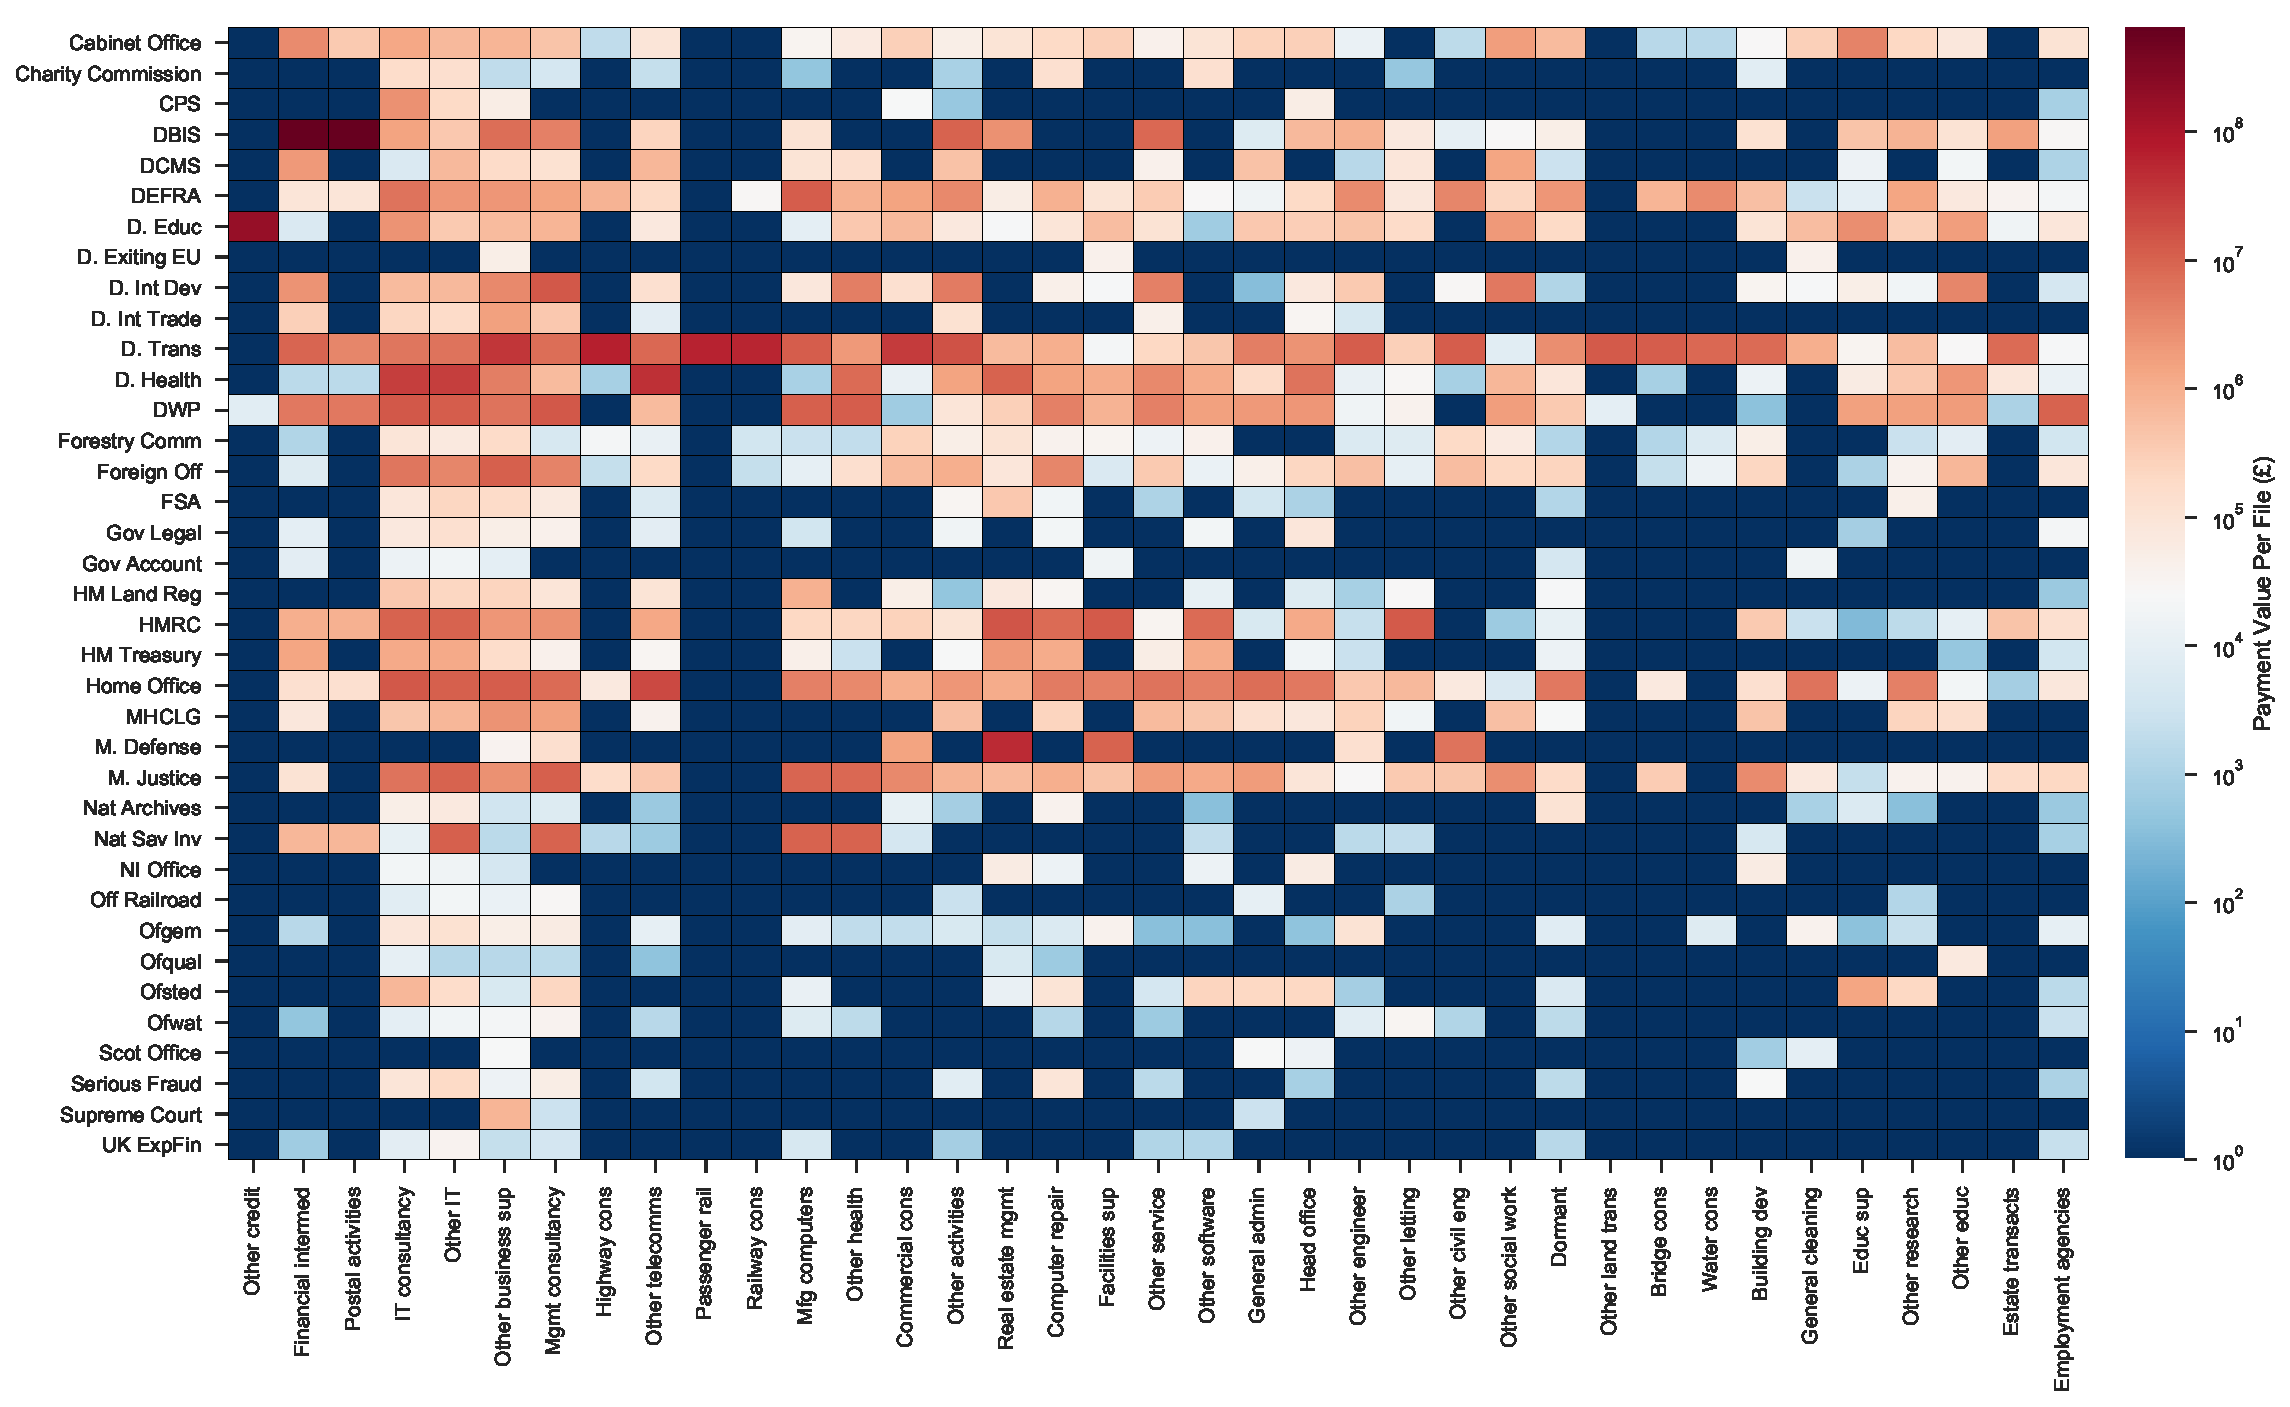
\includegraphics[width=.9\textwidth, angle=0]{sic_dept_heatmap.pdf}
\end{figure}
}

\frame{
\frametitle{Highest Value Private Sector Suppliers (top 20 by value)}
\begin{table}[]
\centering
\label{my-label}\tiny
\begin{tabular}{rccccc}\toprule
Best Match                              & Value ($\pounds$bn) & Number & Postcode & SIC               & Type          \\ \midrule
Student Loans Company           & 16.36       & 27                 & DL1 1RW  & 64929                      & ltd           \\
British Broadcasting Corporation        & 11.98       & 178                & N/A      & N/A & Royal-charter \\
Post Office                     & 9.73        & 1086               & EC2Y 9AQ & Multiple & ltd           \\
Crossrail Limited                       & 4.72  & 27                 & E14 5LQ  & 42120 & ltd           \\
Atos It Services UK             & 2.37 & 10763              & WC1V 6EA & Multiple & ltd\\
Airwave Solutions               & 2.13 & 2004               & SW1E 5LB & 61900                      & ltd           \\
Connect Plus (M25)             & 2.01        & 2662               & EN6 3NP  & 42110                      & ltd           \\
Ibm United Kingdom              & 1.87 & 4663               & PO6 3AU  & 26200                      & ltd           \\
The Arts Council Of England             & 1.68& 61 & N/A  & N/A & royal-charter \\
London \& South Eastern Railway & 1.61 & 242                & NE1 6EE  & 49100                      & ltd \\
BT Group & 1.57	& 732	& EC1A 7AJ	& 61900	& plc\\
Fujitsu Services & 1.47 & 4468 & W1U 3BW & Multiple & ltd \\
Balfour Beatty Civil Engineering & 1.46 & 1807 & E14 5HU & 41201 & ltd \\
Capita Business Services & 1.31 & 26121 & SW1H 0XA & 62020 & ltd \\
Northern Rail & 1.31 & 377 & RG27 9UY & 82990 & ltd\\
Csc Computer Sciences & 1.28 & 1083 & GU11 1PZ & Multiple & ltd \\
Mapeley Steps Contractor & 1.15 & 2779 & WD17 1HP & Multiple & ltd \\
EPSRC & 1.13 & 61 & N/A & N/A & royal-charter\\
High Speed Two (HS2) & 0.98 & 140 & B4 6GA & Multiple & plg-nsc\\
MRC & 0.86 & 129 & N/A & N/A & royal-charter\\ 
$\vdots$ & $\vdots$ & $\vdots$ & $\vdots$ & $\vdots$ & $\vdots$\\ \bottomrule
\end{tabular}
\end{table}
}

\frame{
\frametitle{Grouped by Departments (top 20 by value)}
\begin{table}[]
\centering
\label{my-label}
\tiny
\begin{tabular}{rccccc}\toprule
Department & Files          & Value ($\pounds$m) & Number & \% to Prviate & Most Frequent PS Supplier              \\ \midrule
D. Health      & 47         & 417903         & 60873         & 1.4                       & EXPOTEL HOTEL RESERVATIONS LIMITED \\
D. Trans       & 84         & 149733         & 669722        & 20.62                     & INCHCAPE FLEET SOLUTIONS LIMITED   \\
D. Educ        & 93         & 145867         & 89067         & 12.74                     & REDFERN TRAVEL LIMITED             \\
Home Office    & 112        & 96104.4        & 113659        & 10.43                     & SPECIALIST COMPUTER CENTRES PLC    \\
D. Int Dev     & 88         & 50030.8        & 144439        & 9.56                      & ADAM SMITH INTERNATIONAL LTD       \\
DBIS           & 14         & 41388.9        & 27670         & 32.67                     & CAPITA BUSINESS SERVICES LTD       \\
DWP            & 63         & 23509.7        & 1363930       & 27.14                     & XEROX (UK) LIMITED                 \\
DCMS           & 44         & 18271.4        & 4614          & 78.58                     & BRITISH BROADCASTING CORPORATION   \\
DEFRA          & 62         & 18082.2        & 36603         & 19.34                     & IBM UNITED KINGDOM LIMITED         \\
HMRC           & 95         & 12996.6        & 43359         & 28.41                     & TNT UK LIMITED                     \\
M. Justice     & 42         & 9396.63        & 24155         & 17.13                     & ATOS IT SERVICES UK LIMITED        \\
Foreign Off    & 24         & 4685.37        & 16892         & 28.79                     & FCO SERVICES LTD                   \\
Cabinet Office & 100        & 3308.6         & 14643         & 48.72                     & CAPITA BUSINESS SERVICES LTD       \\
MHCLG          & 2          & 2210.53        & 8553          & 1.2                       & REDFERN TRAVEL LIMITED             \\
Nat Sav Inv    & 93         & 1288.33        & 2532          & 83.84                     & ATOS IT SERVICES UK LIMITED        \\
HM Treasury    & 85         & 1236.09        & 3973          & 40.13                     & FUJITSU SERVICES LIMITED           \\
D. Int Trade   & 20         & 427.29         & 1966          & 35.74                     & GRANT THORNTON UK LLP              \\
Forestry Comm  & 47         & 405.3          & 8865          & 32.86                     & EDF ENERGY 1 LIMITED               \\
CPS            & 49         & 400.63         & 6924          & 38.45                     & CGI IT UK LIMITED                  \\
HM Land Reg    & 62         & 341.17         & 36201         & 70.13                     & CARILLION SERVICES LIMITED  \\
$\vdots$ & $\vdots$ & $\vdots$ & $\vdots$ & $\vdots$ & $\vdots$ \\ \bottomrule
\end{tabular}
\end{table}
}

\section{Social Stratification}

\frame{
\frametitle{A Social Stratification Style Application}
\begin{itemize}
\item This is where the talk about \texttt{centgovspend} ends - hopefully there will be multiple uses for it. At this point we have:\vspace{0.01in}
\begin{enumerate}
\setbeamercolor{enumerate subitem}{fg=red!80!black}
\setbeamertemplate{enumerate items}[default]
\item Cleaned datbase of reonciled government spending. \vspace{0.01in}
\item Database of these suppliers and a confident subset of private sector companies and their characteristics.\vspace{0.01in}
\item A list of officers and PSC associated with all these companies.\vspace{0.01in}
\end{enumerate}
\item Moving to a \textbf{brief} example: a social stratification style application of officers and PSC which are supplying central government relating to:\vspace{0.01in}
\begin{enumerate}
\setbeamercolor{enumerate subitem}{fg=red!80!black}
\setbeamertemplate{enumerate items}[default]
\item Age
\item Gender
\item Nationality and Country of Residence
\item Occupation
\end{enumerate} 
\item We can use the CH PSC flatfile, but had to set up a huge scrape of CH API to build an officers flatfile.
\end{itemize}
}


\frame{
\frametitle{Age of Officers and Persons of Significant Control}
\begin{figure}
\centering
\begin{subfigure}{.5\textwidth}
  \centering
    \caption{Officers}
  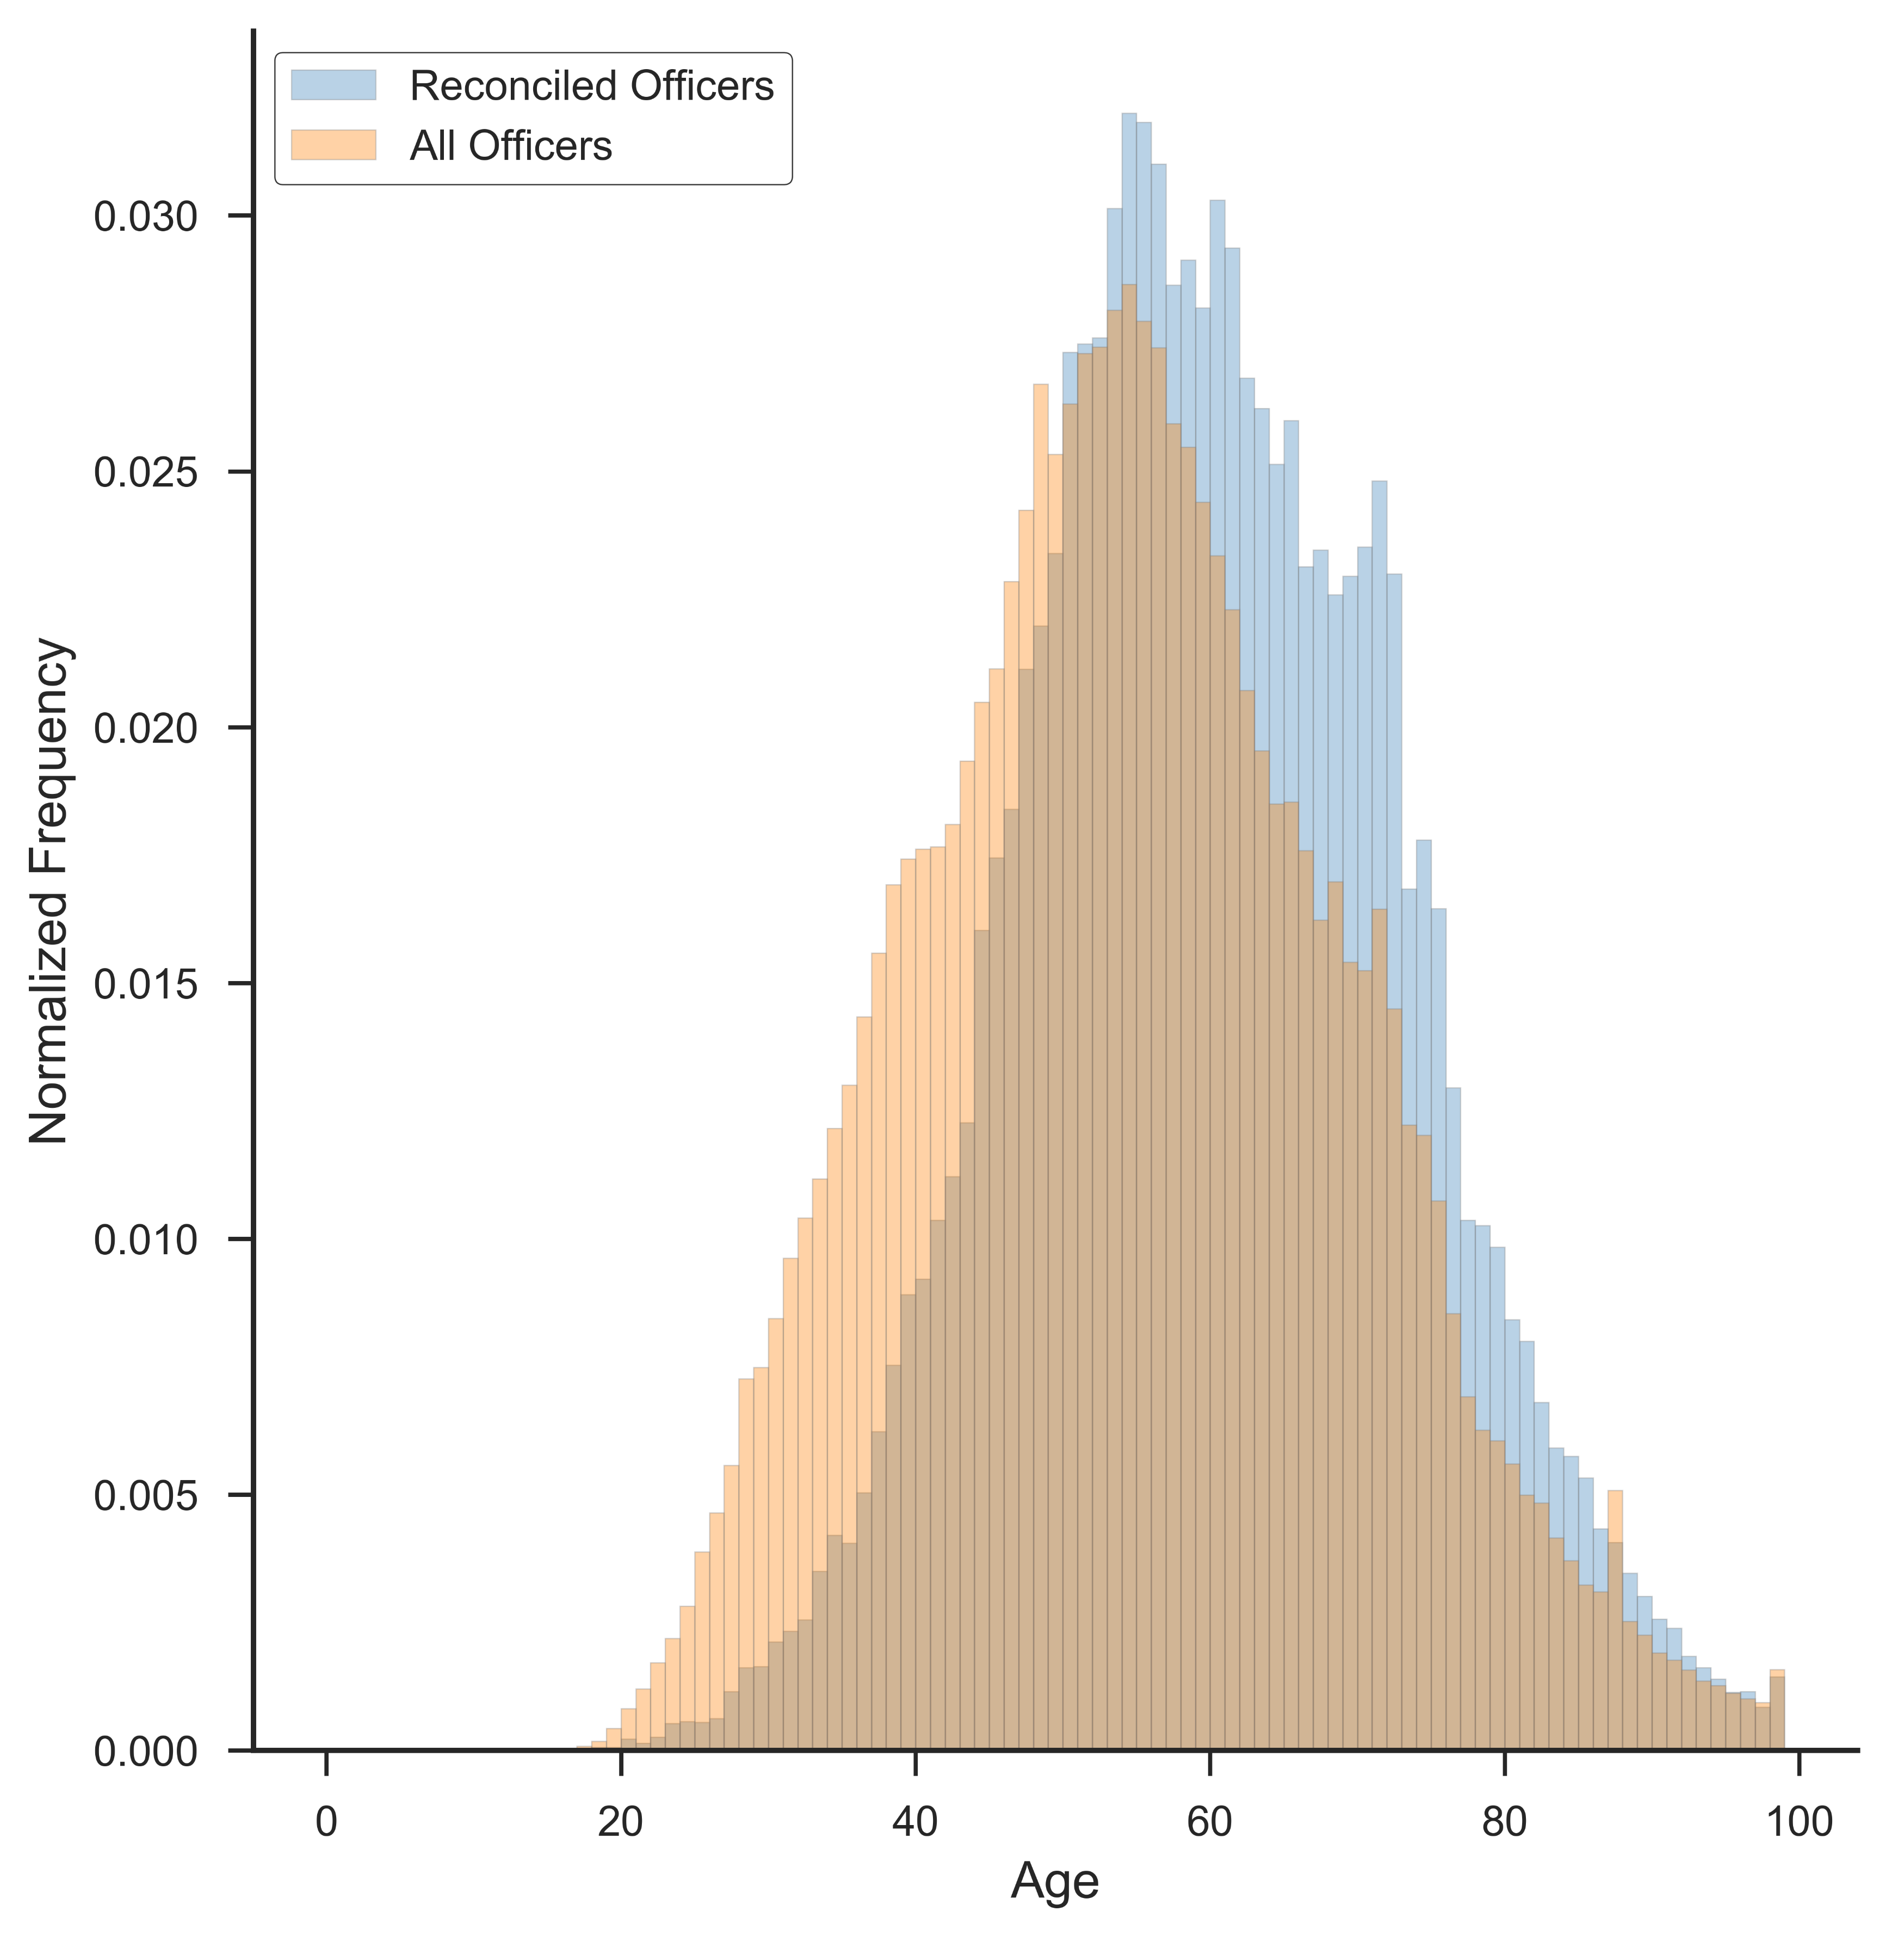
\includegraphics[width=.8\linewidth]{charlie_1.png} 
  \label{fig:sub1}
\end{subfigure}%
\begin{subfigure}{.5\textwidth}
  \centering
    \caption{Persons of Significant Control}
  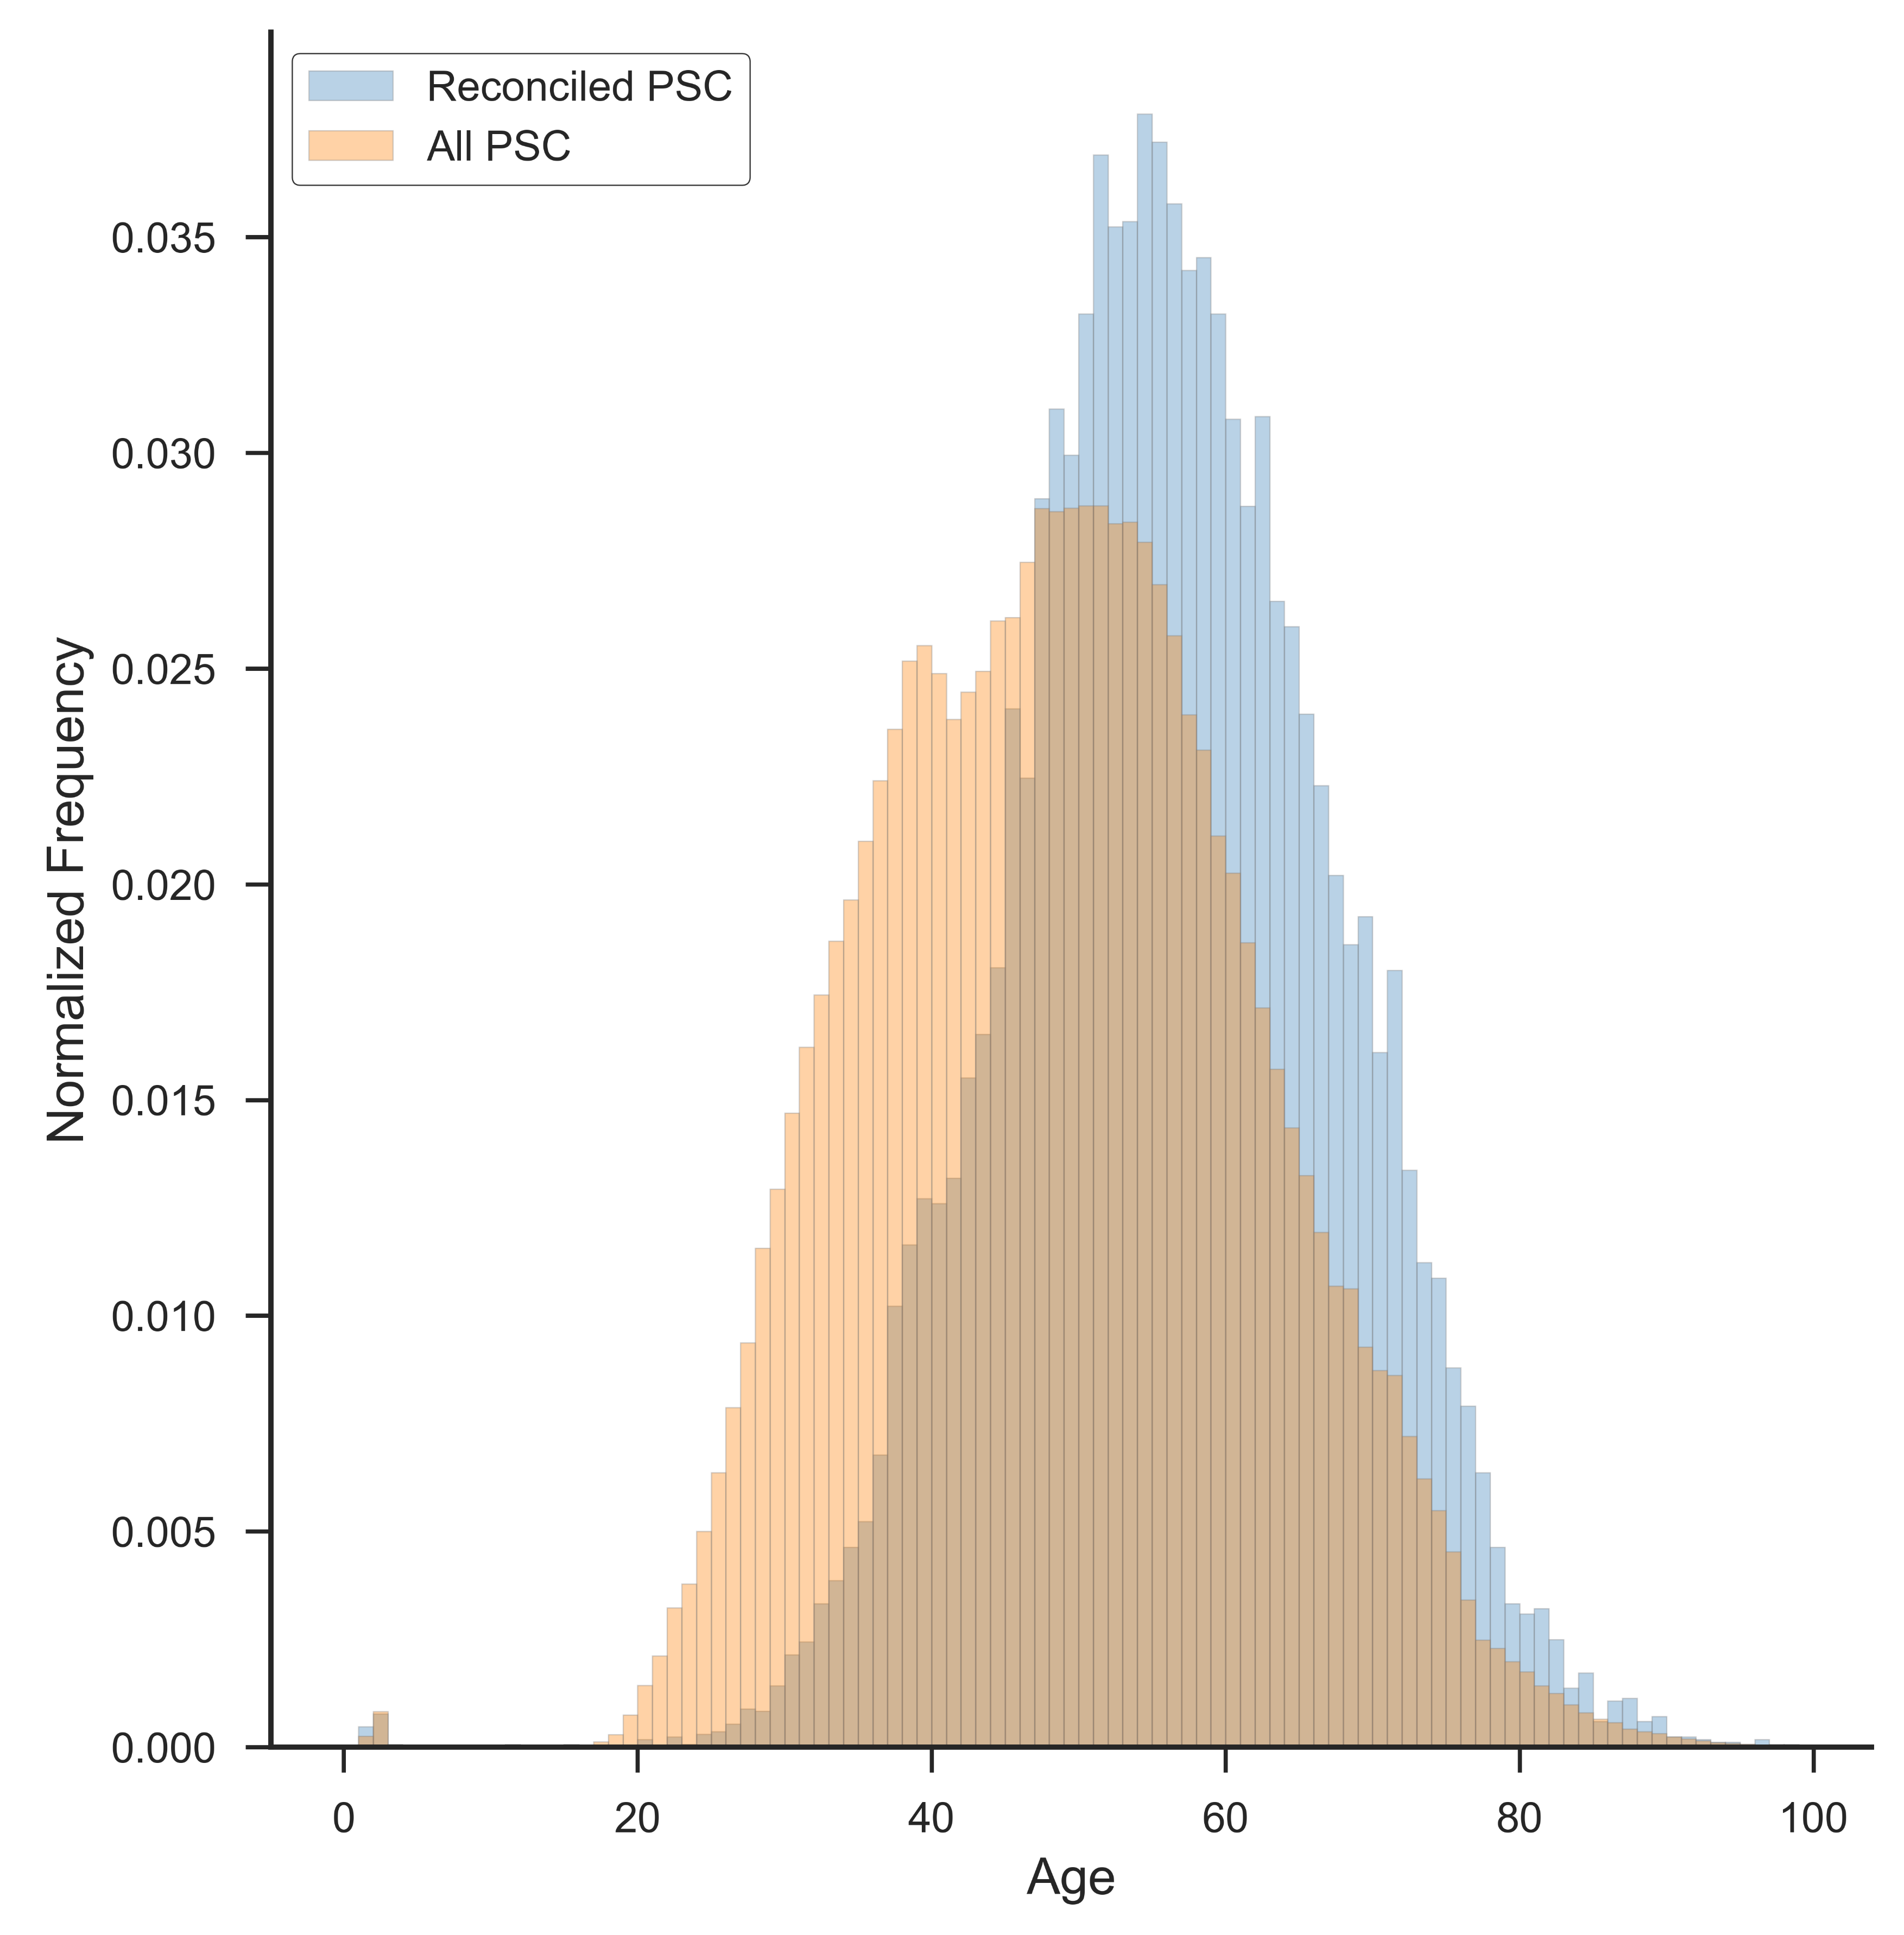
\includegraphics[width=.8\linewidth]{charlie_2.png}
  \label{fig:sub2}
\end{subfigure}
\label{fig:test}
\end{figure}\scriptsize
\begin{itemize}
\item Full CH Officers have an average age of 58: government supplier subset 64.
\item CH PSC have an average age of 56: government supplier subset 62.
\end{itemize}
}

\frame{
\frametitle{Gender}
\begin{itemize}
\item We can also attempt to estimate gender ratios...
\item for officers and PSC in whole of CH and subset of government suppliers.
\item Uses a carefully prepared international name dictionary (\texttt{gender\_guesser}).
\item Generate forenames from splitting names on whitespace, ignoring titles.
\item Drop any returns to androgynous names.
\item Naively appropriate `mostly\_male/female' to `male/female'.
\item Gender ratios are fairly constant between CH and reconciled subset:
\begin{itemize}
\item 29.5\% female officers in entire CH, 28.1\% in reconciled suppliers.
\item 27.8\% female PSC in entire CH, 27.9\% in reconciled suppliers.
\end{itemize}
\item Perhaps most striking here is the global distance from 51\% females.
\end{itemize}
}


\frame{
\frametitle{Internationality of Officers and PSC}
\begin{figure}
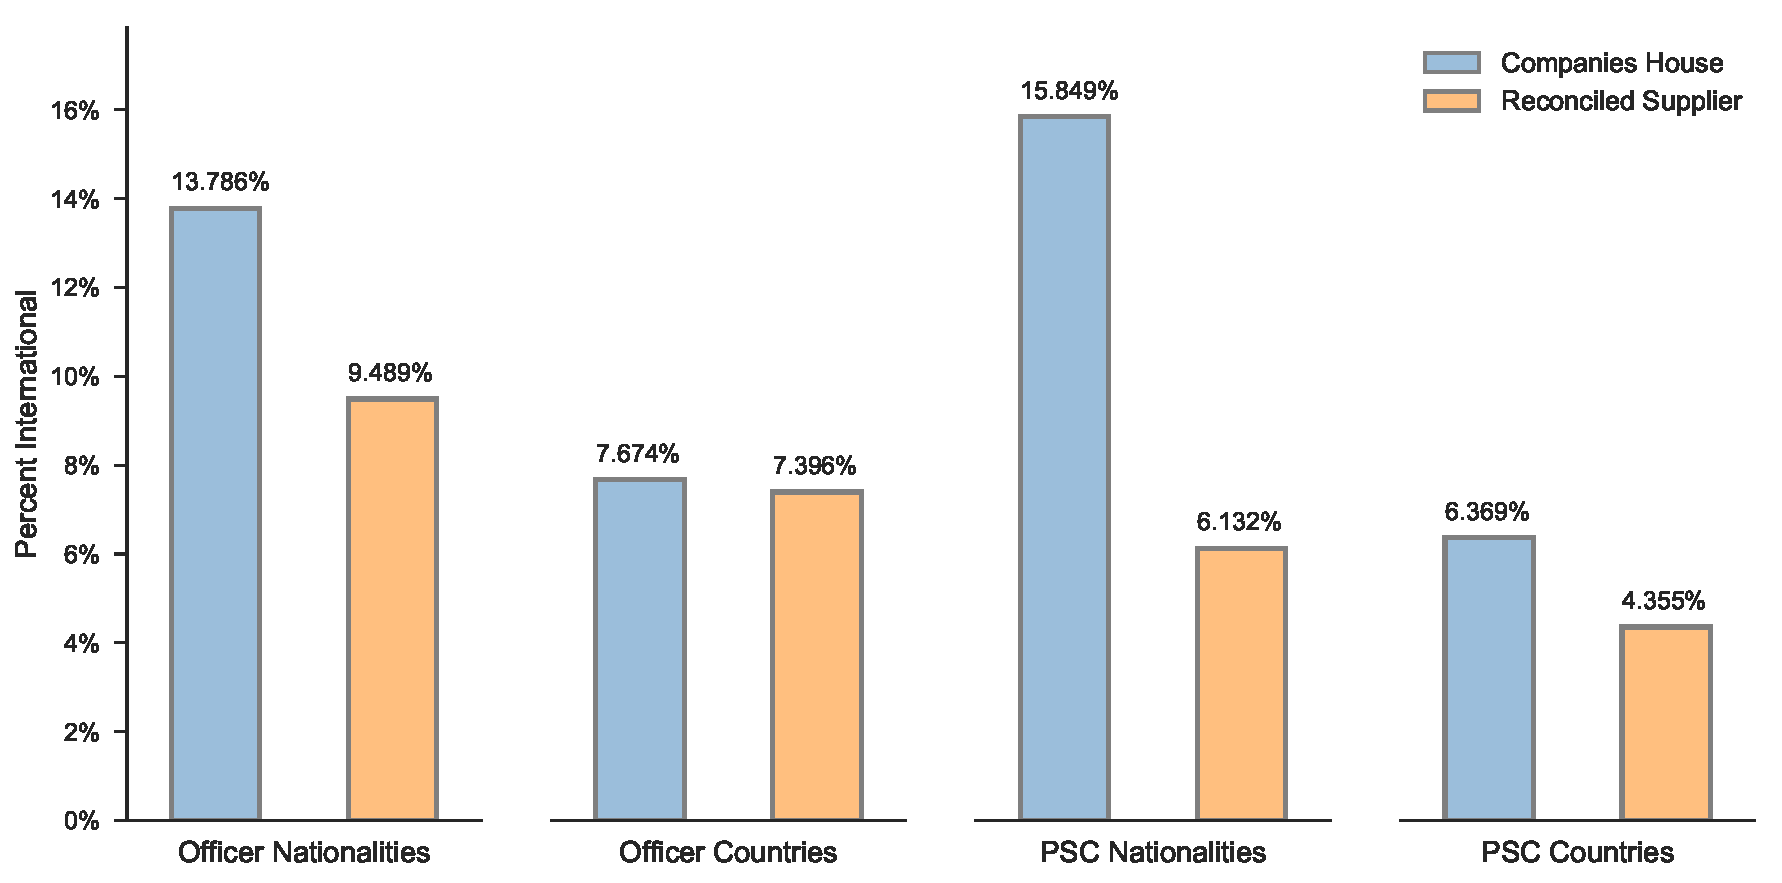
\includegraphics[width=.9\textwidth, angle=0]{countries_and_nationalities.pdf}
\end{figure}
}


\frame{
\frametitle{Occupation}
\begin{figure}
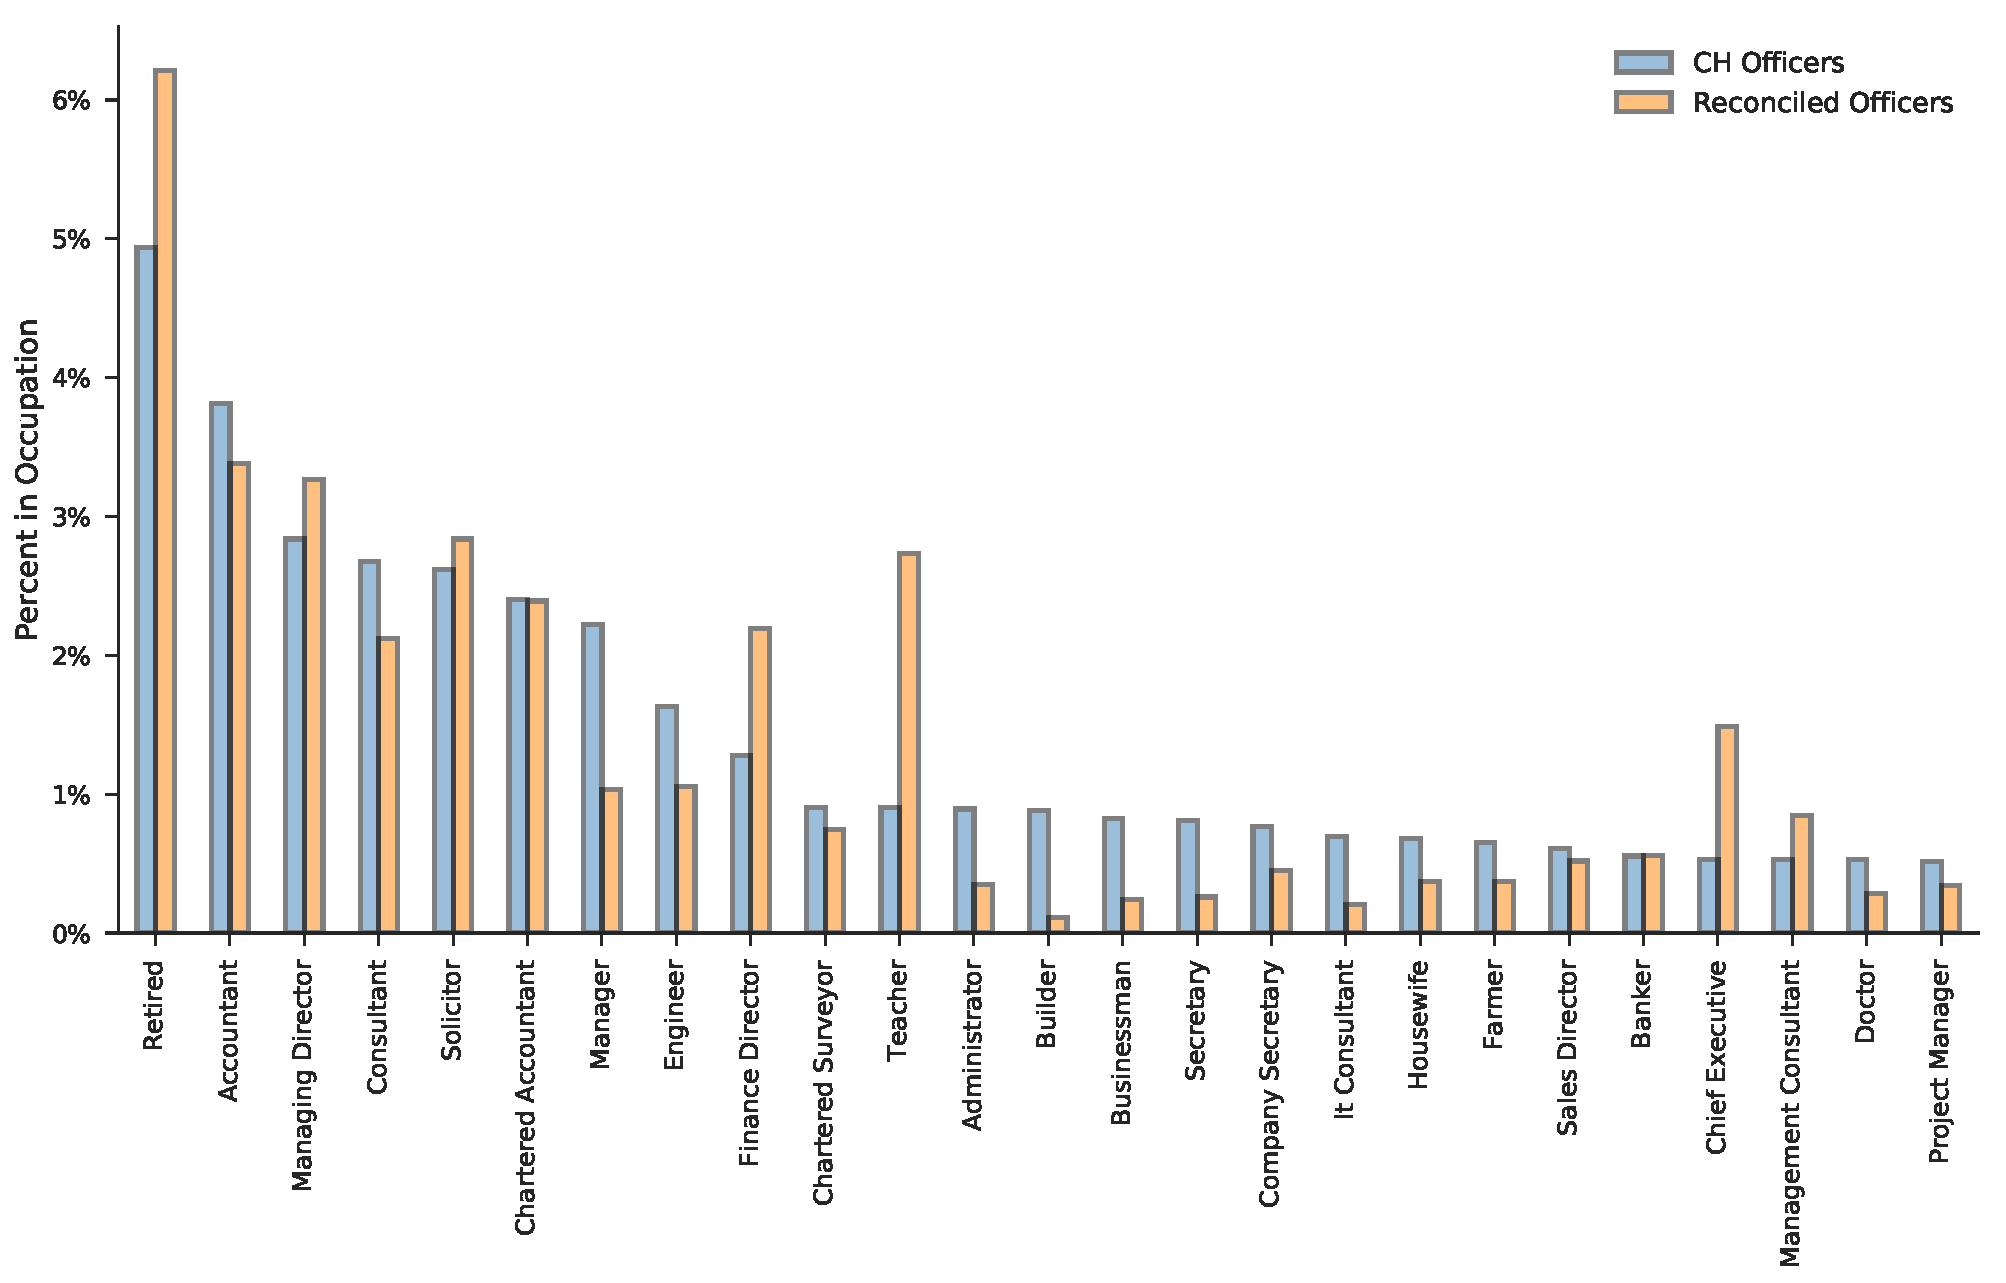
\includegraphics[width=.925\textwidth, angle=0]{officer_occupations.pdf}
\end{figure}
}

\section{Conclusion}
\frame{
\frametitle{Conclusion}
\begin{itemize}
\item This is \textbf{very} much a work in progress! Developments to come:\vspace{0.1in}
\begin{enumerate}
\setbeamercolor{enumerate subitem}{fg=red!80!black}
\setbeamertemplate{enumerate items}[default]
\scriptsize
\item Brush off JavaScript skills and build an online interactive dashboard.\vspace{0.1in}
\item Write ML based algorthm for suggesting better, more consistent redactions.\vspace{0.1in}
\item Develop elastic-search based API for reconciling other (e.g. NHS Digital) registers.\vspace{0.1in}
\item Validate through merges with annual accounting budgets.\vspace{0.1in}
\item Add a third -- national -- dimension of comparisons to officer \& PSC characteristics.\vspace{0.1in}
\item Tidy up the library, unit test, and turn it into a working paper.\vspace{0.1in}
\end{enumerate}
\footnotesize
\item This is hopefully a valueable tool for academic researchers and is still in its inception -- please don't hesitate to get in touch with comments, suggestions or requests for bulk downloads.\vspace{0.05in}
\item Next up: \texttt{NHSspend} (for which this was largely a prototype of).
\end{itemize}

}

\end{document}